\clearpage
\section{Постановка задачи}
В ходе исследования был проведен сравнительный анализ существующих популярных фреймворков (см. табл. \ref{task:comp_table}). Из таблицы видно, что наиболее популярным ускорителем является CUDA. Пркатически с момента релиза Tensorflow сообщество ведет разговоры о поддержке OpenCL\footnote{https://github.com/tensorflow/tensorflow/issues/22}. На сегодняшний день есть очень ограниченная поддержка технологии, реализованная с помощью проприетарной библиотеки ComputeCpp. Кроме того, компания Intel добавила ограниченную поддержку сопроцессоров Movidius\footnote{https://software.intel.com/en-us/neural-compute-stick}, которая позволяет ускорить выполнение сетей, но не их обучение. Наибольших успехов достигла компания Facebook, разрабатывающая библиотеку Glow. Но ее инженеры решили отказаться от использования сторонних библиотек, таких как Intel MKL, Eigen и т.д. Потенциально это может привести к серьезным потерям производительности, так как не всегда компилятор может автоматически задействовать весь доступный набор инструкций.
\par
В связи с вышеизложенными фактами было принято решение разработать собственный фреймворк. Его главными качествами должны стать портируемость, расширяемость и ориентация на достижение высокой производительности.
\par
%\begin{table}
\begin{sidewaystable}
\caption{Сравнительный обзор фреймворков}
\label{task:comp_table}
\begin{tabularx}{\textwidth}{@{}ZZZZZZZ@{}}
\toprule
\textbf{Фреймворк} & \textbf{Лицензия}       & \textbf{Ускорители}                    & \textbf{Модель распределенных вычислений}  & \textbf{Сложность добавления новых операций} & \textbf{Сложность добавления поддержки новой архитектуры} & \textbf{Поддерживаемые ОС}          \\ \midrule
Tensorflow         & Apache 2.0              & CUDA, Google TPU, Qualcomm Hexagon DSP & Сервер параметров                          & Средняя                                      & Высокая                                                   & Windows, Linux, macOS, Android, iOS \\
Caffe              & BSD                     & CUDA                                   & Нет                                        & Высокая                                      & Высокая                                                   & Windows, Linux, macOS               \\
Theano             & Proprietary open source & CUDA                                   & Нет (только с помощью сторонних библиотек) & Низкая                                       & Средняя                                                   & Windows, Linux, macOS               \\
PyTorch            & Proprietary open source & CUDA                                   & Нет (только с помощью сторонних библиотек)  & Средняя                                      & Высокая                                                   & Windows, Linux                      \\
CNTK               & MIT                     & CUDA                                   & Сервер параметров                          & Высокая                                      & Высокая                                                   & Windows, Linux                      \\
Glow               & Apache 2.0              & OpenCL                                 & Нет                                        & Средняя                                      & Низкая                                                    & Windows, Linux, macOS               \\ \bottomrule
\end{tabularx}
\end{sidewaystable}
%\end{table}

\begin{figure}[h]
        \centering
        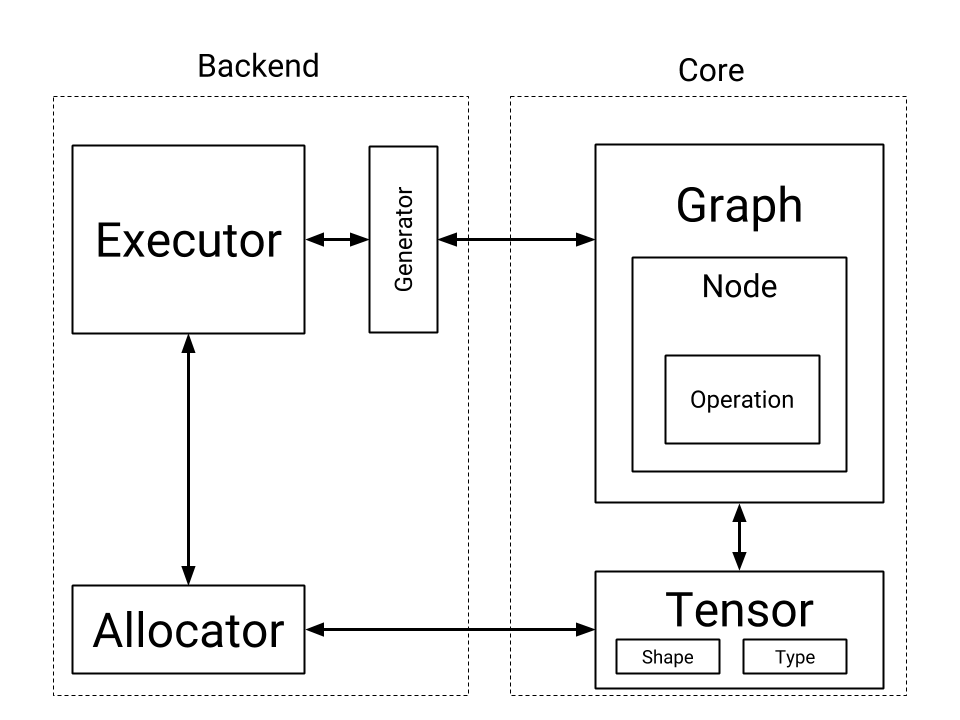
\includegraphics[width=0.8\textwidth]{proj_scheme}
        \caption{Схема проекта}
        \label{task:proj_scheme}
\end{figure}
Структуру фреймворка можно разделить на Backend и Core (см. рис. \ref{task:proj_scheme}). Core - ядро фреймворка. Главная его часть - граф вычислений (Graph). В рамках данной работы под графом вычислений будет пониматься направленный ациклический граф. Он состоит из множества вершин (Node). Вершина может содержать операции (Operation) или тензоры (Tensor). Под тензором будет пониматься многомерный массив, для которого заданы набор размеров каждого измерения (Shape) и тип данных (Data type). Тензор является единицей информации в графе. Каждая операция принимает ноль и более тензоров и возвращает ноль и более тензоров. Таким образом, граф представляет собой функцию многих переменных, для которой необходимо найти глобальный минимум. Ядро - центральный компонент фреймворка, обеспечивающий взаимодействие с остальными частями.
\par
Backend представляет собой абстрактную виртуальную машину. С ее помощью будет исполняться граф вычислений. Фреймворк будет содержать несколько различных виртуальных машин, но все они должны удовлетворять ряду требований. Во-первых, все виртуальные машины должны поддерживать виртуальное адресное пространство (ВАП) на основе линейной модели памяти. Адрес в ВАП является натуральным числом из отрезка [1, $2^{64}-1$]. Адрес 0 является зарезервированным. Распределением памяти в ВАП, а также трансляцией виртуальных адресов фреймворка в реальные\footnote{Под реальными понимаются адреса, характерные для устройства памяти. Например, для оперативной памяти это будет виртуальный адрес из ВАП приложения, который затем будет преобразован в физический адрес средствами ОС.} занимается аллокатор (Allocator). Аллокатор может инкапсулировать в себе механизмы взаимодействия с физической памятью (например, с оперативной памятью или памятью видеокарты), управления подкачкой, распределения виртуальных адресов. У виртуальной машины может быть более одного аллокатора. Например, обучение производится на выделенном сервере, значит, можно использовать всю доступную оперативную память. А исполнение -- на домашнем компьютере пользователя, значит потребление ОЗУ не должно быть чрезмерным. Для этих целей имеет смысл создать два различных аллокатора.
\par
Непосредственно выполнением графа будет заниматься исполнитель (Executor). С помощью генератора он будет получать всю необходимую для исполнения. Он также отвечает за работу с многопоточностью.
В качестве первой виртуальной машины будет использоваться LLVM — универсальная система анализа, трансформации и оптимизации программ, реализующая виртуальную машину с RISC-подобными инструкциями. Может использоваться как оптимизирующий компилятор байткода в машинный код для различных архитектур либо для его интерпретации и JIT-компиляции (для некоторых платформ).
\begin{figure}[h]
	\centering
	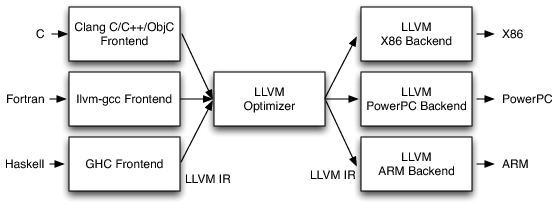
\includegraphics[width=0.75\textwidth]{llvm}
	\caption{Структура компилятора LLVM}
	\label{task:llvm}
\end{figure}
\par
Типичный компилятор на основе LLVM делает лексический разбор исходного кода, строит абстрактное синтаксическое дерево (Abstract Syntax Tree, AST), а затем генерирует LLVM IR - специальное промежуточное представление, которое позже будет преобразовано в машинный код. В случае фреймворка, в качестве AST может выступать граф вычислений. Таким образом, большая часть работы оказывается выполненной.
\begin{figure}[h]
	\centering
	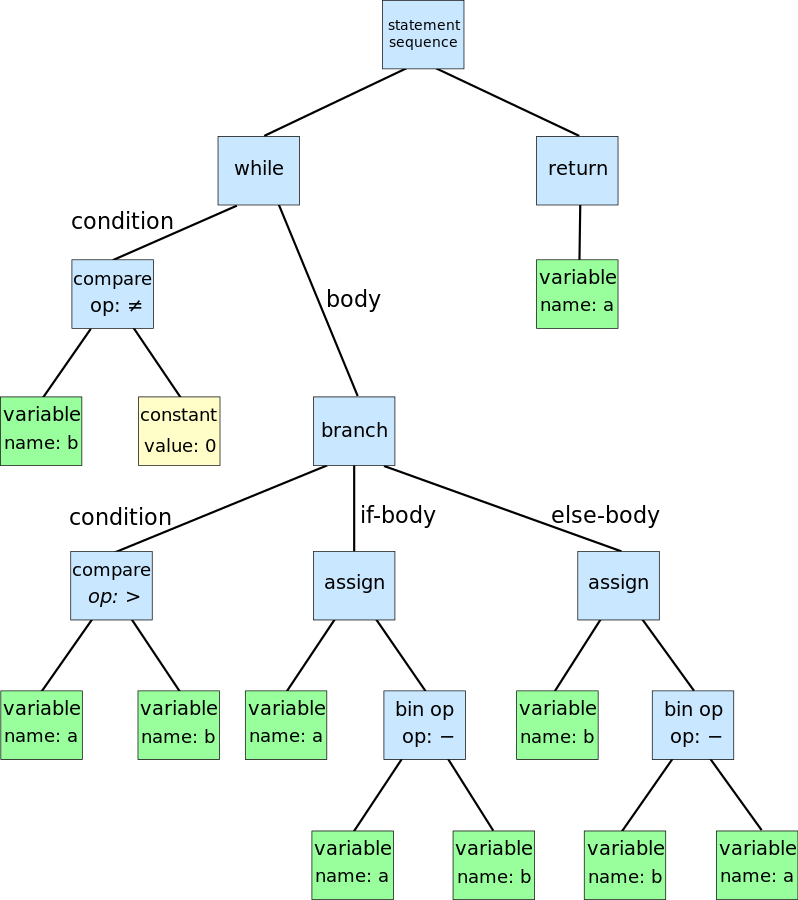
\includegraphics[width=0.6\textwidth]{ast}
	\caption{Абстрактное синтаксическое дерево}
	\label{task:ast}
\end{figure}
\begin{lstlisting}[caption=Псевдокод]
while b != 0
    if a > b
        a := a − b
    else
        b := b − a
return a
\end{lstlisting}
\par
Использование LLVM даст следующие преимущества:
\begin{enumerate}
	\item Быстрая среда исполнения. LLVM позволяет скомпилировать байткод, что дает прирост производительности по сравнению с исполнением графа во время обхода.
	\item Оптимизации. В LLVM встроено множество инструментов для низкоуровневых оптимизаций байткода.
	\item Возможность создать исполняемый файл, который будет содержать только граф вычислений. Это позволит эффективно встраивать обученную модель в пользовательские приложения.
\end{enumerate}
\par
	Одновременное обучение на нескольких устройствах останется перспективой на будущее и не будет рассматриваться в рамках данной работы.
